\documentclass[12pt,a4paper]{article}

% Essential packages
\usepackage[utf8]{inputenc}
\usepackage[T1]{fontenc}
\usepackage[english]{babel}
\usepackage{geometry}
\usepackage{graphicx}
\usepackage{xcolor}
\usepackage{fancyhdr}
\usepackage{titlesec}
\usepackage{tocloft}
\usepackage{booktabs}
\usepackage{amsmath}
\usepackage{amssymb}
\usepackage{listings}
\usepackage{hyperref}
\usepackage{caption}
\usepackage{subcaption}
\usepackage{enumitem}
\usepackage{float}
\usepackage{colortbl}
\usepackage{pgfgantt}
\usepackage{parskip}


% Page geometry
\geometry{
    top=2.5cm,
    bottom=2.5cm,
    left=2.5cm,
    right=2.5cm,
    headheight=15pt
}

% Color definitions
\definecolor{primaryblue}{RGB}{41, 128, 185}
\definecolor{secondaryblue}{RGB}{52, 152, 219}
\definecolor{darkgray}{RGB}{44, 62, 80}
\definecolor{lightgray}{RGB}{149, 165, 166}
\definecolor{accentgreen}{RGB}{39, 174, 96}
\definecolor{codebackground}{RGB}{248, 249, 250}

% Define team member colors
\definecolor{JesusGreen}{HTML}{27ae60}
\definecolor{ArnauPurple}{HTML}{9b59b6}
\definecolor{MarcBlue}{HTML}{2980b9}
\definecolor{MichelRed}{HTML}{e74c3c}
\definecolor{SharedOrange}{HTML}{FFA500}

% Hyperlink setup
\hypersetup{
    colorlinks=true,
    linkcolor=primaryblue,
    filecolor=primaryblue,
    urlcolor=primaryblue,
    citecolor=primaryblue,
    pdftitle={MD-P1-Report},
    pdfauthor={Group 6}
}

% Header and footer setup
\pagestyle{fancy}
\fancyhf{}
\fancyhead[L]{\textcolor{darkgray}{\small Data Mining}}
\fancyhead[R]{\textcolor{darkgray}{\small Group 6}}
\fancyfoot[C]{\textcolor{lightgray}{\thepage}}
\renewcommand{\headrulewidth}{0.5pt}
\renewcommand{\headrule}{\hbox to\headwidth{\color{primaryblue}\leaders\hrule height \headrulewidth\hfill}}

% Title page style
\fancypagestyle{titlepage}{
    \fancyhf{}
    \renewcommand{\headrulewidth}{0pt}
    \renewcommand{\footrulewidth}{0pt}
}

% Section title formatting
\titleformat{\section}
{\Large\bfseries\color{primaryblue}\raggedright}
{\thesection}
{1em}
{}
[\vspace{-0.5em}\textcolor{primaryblue}{\titlerule[1pt]}]

\titleformat{\subsection}
{\large\bfseries\color{secondaryblue}}
{\thesubsection}
{1em}
{}

\titleformat{\subsubsection}
{\normalsize\bfseries\color{darkgray}}
{\thesubsubsection}
{1em}
{}

% Table of contents styling
\renewcommand{\cftsecfont}{\color{primaryblue}\bfseries}
\renewcommand{\cftsubsecfont}{\color{secondaryblue}}
\renewcommand{\cftsecpagefont}{\color{primaryblue}\bfseries}
\renewcommand{\cftsubsecpagefont}{\color{secondaryblue}}

% Code listing setup
\lstdefinestyle{mystyle}{
    backgroundcolor=\color{codebackground},
    commentstyle=\color{lightgray},
    keywordstyle=\color{primaryblue},
    numberstyle=\tiny\color{lightgray},
    stringstyle=\color{accentgreen},
    basicstyle=\ttfamily\footnotesize,
    breakatwhitespace=false,
    breaklines=true,
    captionpos=b,
    keepspaces=true,
    numbers=left,
    numbersep=5pt,
    showspaces=false,
    showstringspaces=false,
    showtabs=false,
    tabsize=2,
    frame=single,
    frameround=tttt,
    rulecolor=\color{lightgray}
}
\lstset{style=mystyle}

% Custom title page commands
\title{}
\author{}
\date{}


\begin{document}

% Custom title page
\thispagestyle{titlepage}
\begin{center}

% Top spacing

% Main title with decorative elements
{\color{primaryblue}\rule{\textwidth}{2pt}}
\vspace{0.5cm}

{\Huge\bfseries\color{primaryblue} DATA MINING}
\vspace{0.3cm}

{\LARGE\color{secondaryblue} Food Marketing}
\vspace{0.5cm}

{\color{primaryblue}\rule{\textwidth}{2pt}}

\vspace{1.5cm}

% Project identifier
{\Large\bfseries\color{darkgray} P1-Report}

\vspace{2cm}

% Group information
{\large\bfseries\color{primaryblue} Group 6}

\vspace{1cm}

% Team members in a nice box
\fcolorbox{primaryblue}{white}{
\begin{minipage}{0.7\textwidth}
\centering
\vspace{0.5cm}
{\large\bfseries\color{primaryblue} Team Members}
\vspace{0.5cm}

\begin{tabular}{@{}c@{}}
\textcolor{darkgray}{Font I Cabarrocas, Marc} \\[0.3cm]
\textcolor{darkgray}{Garcia Ayala, Jesus} \\[0.3cm]
\textcolor{darkgray}{Hernández Navarro, Arnau} \\[0.3cm]
\textcolor{darkgray}{Mediavilla Jiménez, Alex Michel} \\
\end{tabular}
\vspace{0.5cm}
\end{minipage}
}

\vspace{1.5cm}

% Teacher information
{\large\bfseries\color{secondaryblue} Professor}
\vspace{0.3cm}

{\large\color{darkgray} Sergi Ramirez Mitjans}

\vspace{2cm}

% Date
{\large\color{lightgray} \today}

\vspace{1cm}

% Bottom decorative line
{\color{primaryblue}\rule{0.5\textwidth}{1pt}}

\end{center}
\newpage
\tableofcontents
\newpage

\section{Motivation}
Understanding consumer behaviour is crucial in the highly competitive food and grocery market. Consumers exhibit diverse preferences, purchasing habits, and responses to marketing efforts, influenced by demographic factors, lifestyle choices, and economic conditions. Analysing customer data allows businesses to move beyond generic strategies and tailor their offerings, promotions, and communication channels effectively. By uncovering patterns in how different customer groups interact with products (like wine, meat, fruit) and purchase channels (web, store, catalogue), we can gain valuable insights to enhance customer satisfaction, optimize marketing spend, and drive business growth. This project aims to dissect a rich dataset of customer interactions with a food retailer to reveal these underlying structures.


The primary problem addressed in this analysis is the identification and characterization of distinct customer segments within the provided food retail dataset (ifood\_enriched.csv).

While the raw data provides individual details, it's challenging to grasp the overarching patterns and group dynamics. Simply looking at averages or individual variables doesn't reveal how these attributes combine to form coherent customer profiles.

Therefore, the core task is to reduce the complexity of this multi-dimensional data and group similar customers together. We aim to answer questions like:

\begin{itemize}
    \item Are there natural groupings of customers based on their spending habits and demographics?
    \item What are the key characteristics that define these different customer segments?
    \item How do purchasing channel preferences differ across segments?
    \item Can we identify high-value vs. low-value segments, or perhaps niche groups with specific preferences?
\end{itemize}

The ultimate goal is to generate actionable insights by creating well-defined customer profiles based on the identified clusters. These profiles can then inform targeted marketing strategies, personalized recommendations, inventory management, and overall business decision-making for the food retailer

\newpage
\section{Data Source}
The dataset used in this project was obtained from Kaggle, an online platform for data science competitions and open datasets. Specifically, it comes from the dataset “Marketing Data” uploaded by Jack Daoud. The dataset contains customer information, including demographic details, purchasing behaviour, and responses to marketing campaigns, which makes it suitable for customer segmentation and predictive modelling.

% JESUS
%%%%%%%%%%%%%%%%%%%%%%%%%%%%%%%%%%%%%%%%%%%%%%%%%%%%%%%%%%%%%%%%%%%%%%%%%%%%%%%%%
\newpage
\input{metadata.tex}


% ARNAU
%%%%%%%%%%%%%%%%%%%%%%%%%%%%%%%%%%%%%%%%%%%%%%%%%%%%%%%%%%%%%%%%%%%%%%%%%%%%%%%%%
\newpage
\documentclass{article}
\usepackage{graphicx}
\usepackage{pgffor}
\usepackage{pdfpages}
\usepackage{geometry}
\geometry{margin=0pt} % quita márgenes
\usepackage{float}


\begin{document}

\foreach \i in {1,...,35}{%
    \clearpage
    \begingroup
      \edef\FileName{Imatges/d\i.png}%
      \begin{figure}[H]
        \centering
        \includegraphics[width=0.9\linewidth]{\FileName}
      \end{figure}
    \endgroup
}

\paragraph{{Final data description}}
The iFood dataset includes 2,031 customers across nine variables, showing no missing data and excellent quality. Customers are predominantly middle-aged and well-educated, with a wide but reasonable income range (mean €52,844). Family structures are typically small, and complaints are extremely rare (0.98\%). Income relates positively to education and age but negatively to having children, while higher-income, recently active customers respond more to marketing campaigns. Overall, the data are well-behaved, balanced across variables, and suitable for multivariate modeling, with only one extreme income outlier and an imbalanced “Complain” variable as minor considerations.

\end{document}


% MARC
%%%%%%%%%%%%%%%%%%%%%%%%%%%%%%%%%%%%%%%%%%%%%%%%%%%%%%%%%%%%%%%%%%%%%%%%%%%%%%%%%
\newpage
\section{PCA}
Principal Component Analysis (PCA) was performed on the selected numerical variables to reduce dimensionality and identify the main axes of variation within the customer data. The analysis focuses on understanding the underlying structure defined by customer demographics and purchasing behaviour.

The inertia (variance) explained by each principal component is visualized bellow.

\begin{figure}[H]
    \centering
    \includegraphics[width=0.8\linewidth]{Imatges/represented_inertia_plot.pdf}
    \caption{Scree plot showing eigenvalues (variance) of each principal component}
    \label{fig:scree_plot}
\end{figure}

\begin{figure}[H]
    \centering
    \includegraphics[width=0.8\linewidth]{Imatges/cummulated_inertia_plot.pdf}
    \caption{Cumulative explained variance by principal components}
    \label{fig:cumulative_variance}
\end{figure}

Figure \ref{fig:scree_plot} shows the percentage of variance explained by each component individually. PC1 clearly dominates, capturing 37.5\% of the variance.

Figure \ref{fig:cumulative_variance} shows the cumulative variance explained. Based on Kaiser's criterion (eigenvalues > 1, corresponding to components explaining more variance than an average original variable), to avoid excessive combinations, the first four principal components are selected for potential analysis. These four components cumulatively explain 63.3\% of the total variance and will help us determine which dimensions to focus on.

\subsection{Finding a Subspace}

To determine a subspace, a combination of the first four spaces, the ones with most variance will be plotted against one another.

% Individual factor maps - individual figures
\begin{figure}[H]
    \centering
    \includegraphics[width=0.8\linewidth]{Imatges/individuals_map_1_2.pdf}
    \caption{Individual factor map for dimensions 1 and 2}
    \label{fig:individuals_map_1_2}
\end{figure}

\begin{figure}[H]
    \centering
    \includegraphics[width=0.8\linewidth]{Imatges/individuals_map_1_3.pdf}
    \caption{Individual factor map for dimensions 1 and 3}
    \label{fig:individuals_map_1_3}
\end{figure}

\begin{figure}[H]
    \centering
    \includegraphics[width=0.8\linewidth]{Imatges/individuals_map_1_4.pdf}
    \caption{Individual factor map for dimensions 1 and 4}
    \label{fig:individuals_map_1_4}
\end{figure}

\begin{figure}[H]
    \centering
    \includegraphics[width=0.8\linewidth]{Imatges/individuals_map_2_3.pdf}
    \caption{Individual factor map for dimensions 2 and 3}
    \label{fig:individuals_map_2_3}
\end{figure}

\begin{figure}[H]
    \centering
    \includegraphics[width=0.8\linewidth]{Imatges/individuals_map_2_4.pdf}
    \caption{Individual factor map for dimensions 2 and 4}
    \label{fig:individuals_map_2_4}
\end{figure}

\begin{figure}[H]
    \centering
    \includegraphics[width=0.8\linewidth]{Imatges/individuals_map_3_4.pdf}
    \caption{Individual factor map for dimensions 3 and 4}
    \label{fig:individuals_map_3_4}
\end{figure}

It's concluded that the planes who will be used for further research are \textbf{PC1-PC2} and \textbf{PC1-PC3}

\newpage

\subsection{Numerical Variables Projection}

% Numerical variables maps PC1-PC2
\begin{figure}[H]
    \centering
    \includegraphics[width=0.9\linewidth]{Imatges/numerical_variables_map_1_2.pdf}
    \caption{Numerical variables correlation circle for dimensions 1 and 2}
    \label{fig:numerical_map_1_2}
\end{figure}

\begin{figure}[H]
    \centering
    \includegraphics[width=0.9\linewidth]{Imatges/numerical_variables_map_1_3.pdf}
    \caption{Numerical variables correlation circle for dimensions 1 and 3}
    \label{fig:numerical_map_1_3}
\end{figure}

From Figure \ref{fig:numerical_map_1_2}, we can observe that the first dimension (PC1) is strongly positively correlated with variables like \texttt{Income}, \texttt{WineExp}, \texttt{MeatExp}, and other expenditure variables. Most variables point to the right side of the plot, indicating they all contribute to the same dimension of customer value.

In Figure \ref{fig:numerical_map_1_3}, we see that \texttt{Age} has a strong positive correlation with PC3, while \texttt{CustDays} has a negative correlation, indicating these variables define opposite sides of the third principal component.

\newpage
\subsection{Qualitative Variables Projection}

The following analysis examines the positions of the illustrative qualitative variables on the factorial maps defined by PC1-PC2 and PC1-PC3. The variables are grouped thematically to build a coherent narrative around the customer profiles.

\begin{figure}[H]
    \centering
    \includegraphics[width=0.9\linewidth]{Imatges/qualitative_modalities_map_1_2.pdf}
    \caption{Qualitative modalities map for dimensions 1 and 2}
    \label{fig:qualitative_map_1_2}
\end{figure}

\begin{figure}[H]
    \centering
    \includegraphics[width=0.9\linewidth]{Imatges/qualitative_modalities_map_1_3.pdf}
    \caption{Qualitative modalities map for dimensions 1 and 3}
    \label{fig:qualitative_map_1_3}
\end{figure}

\newpage
\subsubsection{Core Demographics}

This group of variables describes the fundamental socio-economic profile of the customers.

\begin{itemize}
    \item \textbf{IncomeSegment:} This variable is one of the strongest interpreters of Axis 1 (Customer Value). The \texttt{High} income category is located far to the right (positive on PC1) in Figure \ref{fig:qualitative_map_1_2}, strongly associating it with the high-spending numerical variables (\texttt{Income}, \texttt{WineExp}, \texttt{MeatExp}). Conversely, the \texttt{Low} income category is positioned on the far left (negative on PC1). This confirms that PC1 is a primary axis of economic differentiation. Interestingly, the \texttt{Medium} income category is positioned in the upper half of the plot (positive on PC2), suggesting a link between mid-tier earners and the ``Deal-Seeking Parent of Teens'' profile.
    
    \item \textbf{Education:} The education categories are spread across the map. \texttt{Basic} is located far to the left, aligning with the \texttt{Low} income segment and lower overall customer value. \texttt{Graduation} sits near the center, representing the average customer profile. \texttt{PhD} and \texttt{Master} are positioned slightly in the upper half of the plot, suggesting a weak correlation between higher education and the ``Lifestage'' axis (PC2).
    
    \item \textbf{MaritalSts:} Most marital status categories (\texttt{Married}, \texttt{Together}, \texttt{Single}) are located near the origin, indicating they are not strong differentiators on their own. The one exception is \texttt{Widow}, which is positioned on the right side of the plot (positive on PC1) and slightly in the lower half (negative on PC2). This aligns perfectly with the ``Established, Traditional Shopper'' who is also a higher-value customer.
\end{itemize}

\subsubsection{Household Composition}

This group is crucial for understanding the lifestage of the customers, which strongly defines Axis 2.

\begin{itemize}
    \item \textbf{Kidhome \& HasChildren:} These variables are powerful interpreters of Axis 1. The presence of young children (\texttt{Kidhome 1}, \texttt{HasChildren 1}) is strongly associated with the left side of the plot (negative on PC1), aligning with the low-value customer segment. This suggests that households with young children may have less disposable income for luxury food items. Conversely, \texttt{Kidhome 0} and \texttt{HasChildren 0} are on the right, strongly correlating with the high-value segment.
    
    \item \textbf{Teenhome:} This variable is the single strongest interpreter of Axis 2 (Lifestage \& Channel Preference) as seen in Figure \ref{fig:qualitative_map_1_2}. Having one or two teenagers (\texttt{Teenhome 1}, \texttt{Teenhome 2}) places a customer profile firmly in the upper half of the plot (positive on PC2), aligning perfectly with deal-seeking and web purchases. \texttt{Teenhome 0} is located in the bottom half, associated with the more traditional shoppers. This variable shows almost no correlation with the value axis (PC1), indicating that the presence of teens influences how people shop, but not necessarily how much they spend overall.
\end{itemize}

\subsubsection{Customer Engagement \& Preferences}

This group describes the customers' relationship with the brand and their explicit tastes.

\begin{itemize}
    \item \textbf{CustomerSegment:} This variable serves as an excellent validation of the PCA. \texttt{Segment 2} is positioned on the far right, perfectly aligning with the high-value characteristics of PC1. \texttt{Segment 1} and \texttt{Segment 3} are on the far left, aligning with the low-value profile. The PCA has successfully rediscovered the underlying patterns that were likely used to create these segments in the first place.
    
    \item \textbf{PreferredProductCategory:} The product preferences add nuance to the spending habits. \texttt{WineExp} and \texttt{MeatExp} are positioned on the right (positive on PC1), confirming they are preferred by high-value customers. Other categories like \texttt{FruitExp} and \texttt{SweetExp} are on the left, associated with the lower-value segment.
    
    \item \textbf{PreferredChannel:} Channel preference helps define both axes. \texttt{CatalogPurc} is on the right side (positive on PC1) and slightly in the lower half (negative on PC2), strongly profiling the high-value, established shopper. \texttt{DealsPurc} is at the very top of the plot (highly positive on PC2), confirming its association with the ``Parent of Teens'' lifestage. \texttt{WebPurc} is also in the upper half, while \texttt{StorePurc} is close to the center, indicating it is a general channel used by all segments.
\end{itemize}

Looking at Figure \ref{fig:qualitative_map_1_3}, we can observe additional insights regarding the PC1-PC3 plane. The distribution of qualitative variables along PC3 provides further nuance to our understanding of customer profiles, particularly regarding age and customer tenure relationships.


\subsection{Conclusions}

Based on the variable projections, the principal components can be interpreted as follows:

\begin{itemize}
    \item \textbf{Axis 1 (PC1: 37.5\%): Customer Value.} The positive side (right) is strongly associated with higher \texttt{Income}, higher spending across most categories (especially \texttt{WineExp}, \texttt{MeatExp}, \texttt{CatalogPurc}), and \texttt{CustomerSegment 2}. The negative side (left) corresponds to lower income, lower spending, \texttt{CustomerSegment 1} \& \texttt{3}, and having younger children (\texttt{Kidhome 1}). This axis primarily differentiates customers based on their overall economic value and engagement.
    
    \item \textbf{Axis 2 (PC2: 10.6\%): Lifestage \& Channel Preference.} The positive side (top) is strongly characterized by \texttt{DealsPurc} and \texttt{WebPurc}, along with having teenagers at home (\texttt{Teenhome 1}, \texttt{Teenhome 2}). The negative side (bottom) is associated with having no children or teens (\texttt{HasChildren 0}, \texttt{Teenhome 0}) and potentially more traditional purchasing (\texttt{CatalogPurc}). This axis differentiates customers based on their life stage (presence of teens) and their preferred shopping channels and deal sensitivity.
    
    \item \textbf{Axis 3 (PC3: 8.0\%): Customer Maturity \& Tenure.} The positive side (top) is strongly characterized by higher \texttt{Age}. The negative side (bottom) is associated with longer customer tenure (\texttt{CustDays}). This axis appears to differentiate customers based on their age and how long they have been a customer, potentially contrasting older, perhaps newer high-value customers from younger, more established ones.
\end{itemize}


\newpage
\section{Clustering}
The clustering process begins with the generation of a dendrogram using Ward's method, which minimizes within-cluster variance and produces more balanced clusters. This approach is particularly suitable for customer segmentation as it identifies natural groupings based on similar characteristics.

\begin{figure}[H]
    \centering
    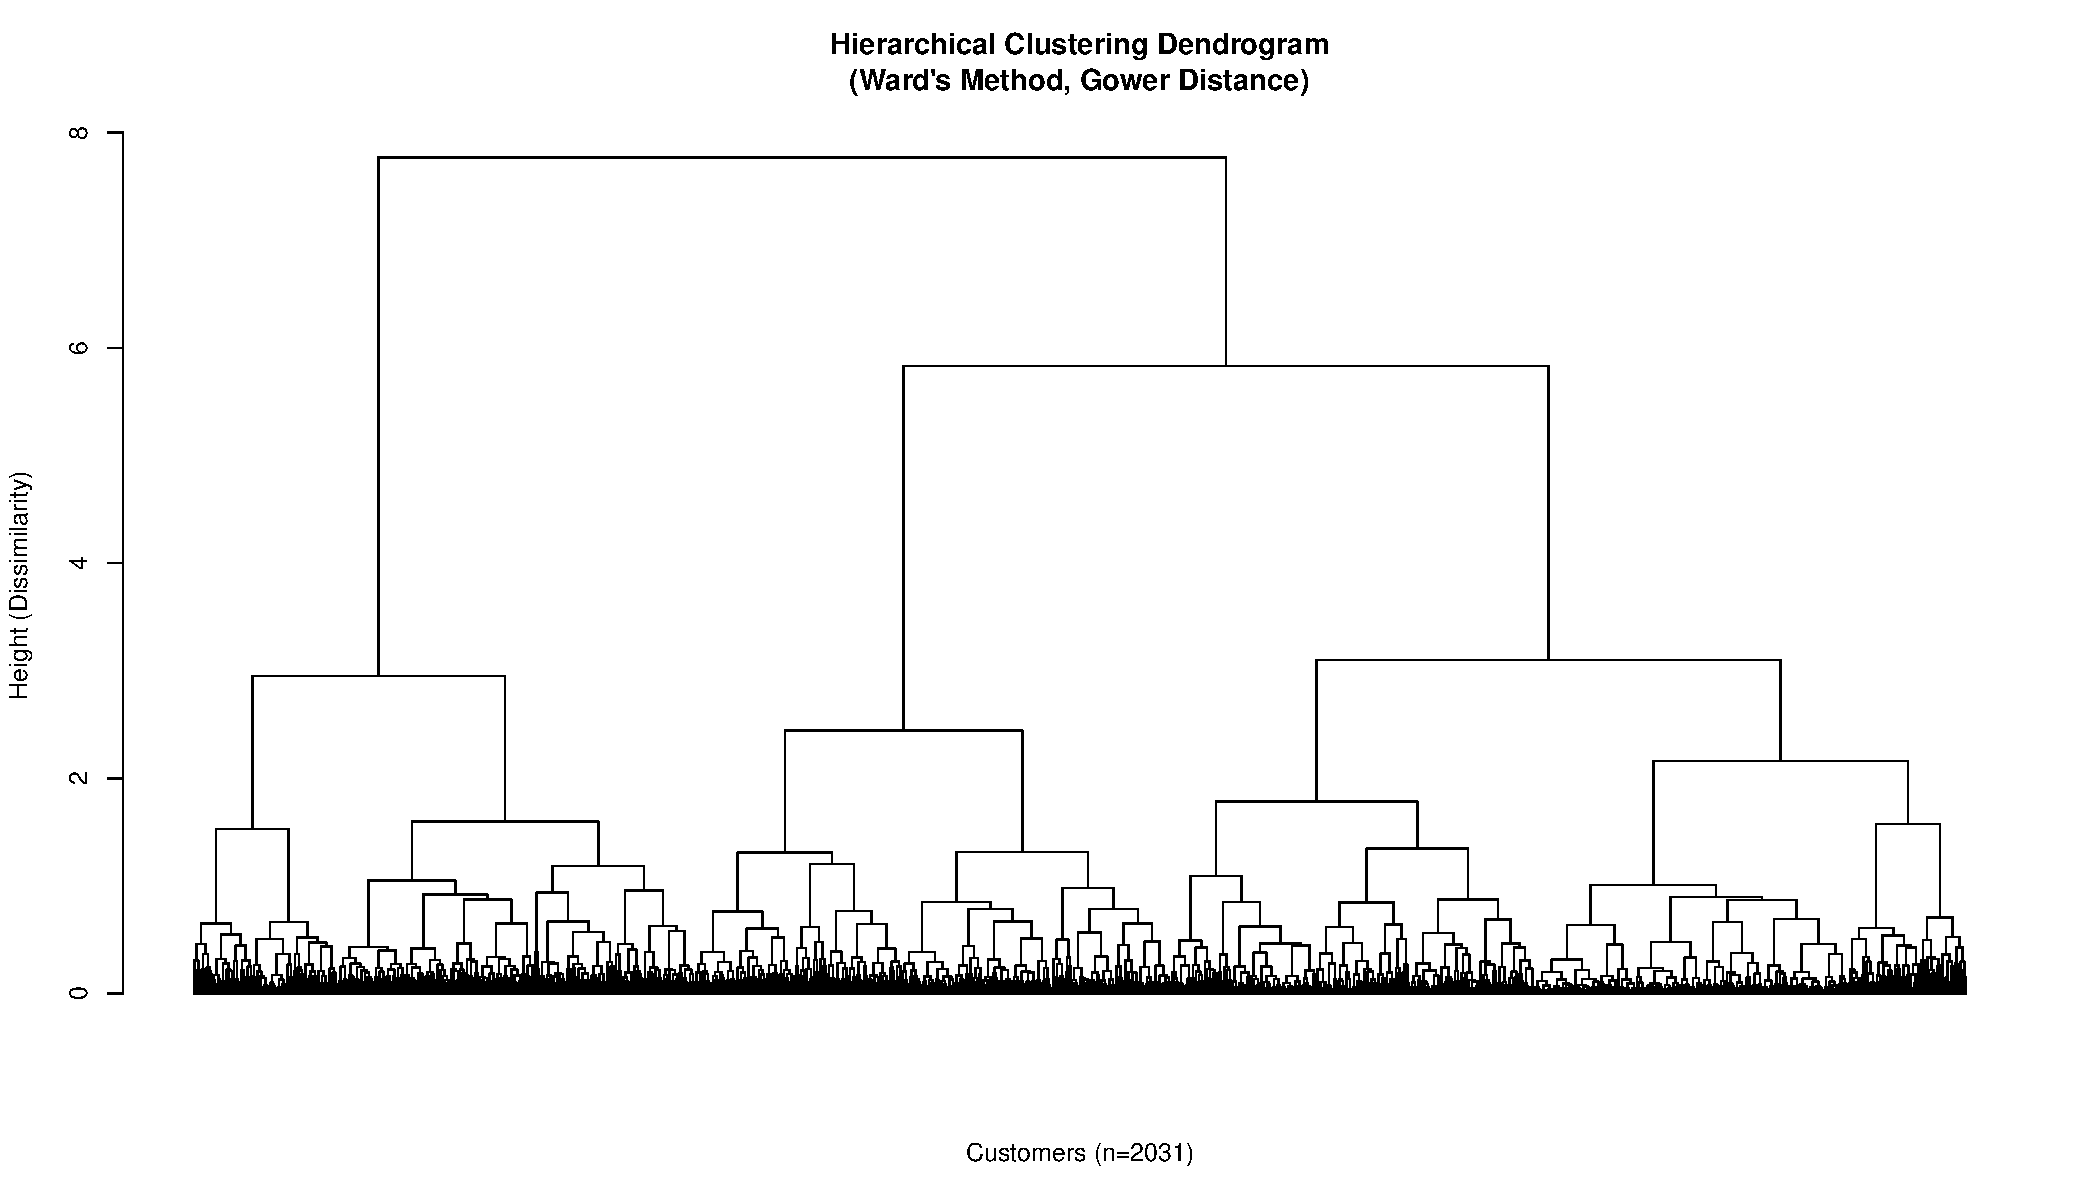
\includegraphics[width=1\linewidth]{Imatges/dendrogram_Gower_Ward.pdf}
    \caption{Dendrogram}
    \label{fig:dend}
\end{figure}

The analysis employed the Gower distance metric to accommodate both numerical variables (income, age, purchase frequency) and categorical variables (education level, marital status) in the dataset. This metric is particularly valuable for mixed data types as it standardizes different variable types into a unified dissimilarity matrix.

Using the elbow method and silhouette analysis shown in Figure \ref{fig:optdig}, it was determined that $k = 3$ is the appropriate number of clusters. The elbow method examines the decrease in within-cluster variation as more clusters are added, with the "elbow" indicating the point of diminishing returns. While silhouette analysis suggested a potential optimum at k = 2, the elbow method showed a notable bend at k = 3, providing better granularity for marketing objectives without over-fragmenting the customer base.

\begin{figure}[H]
    \centering
    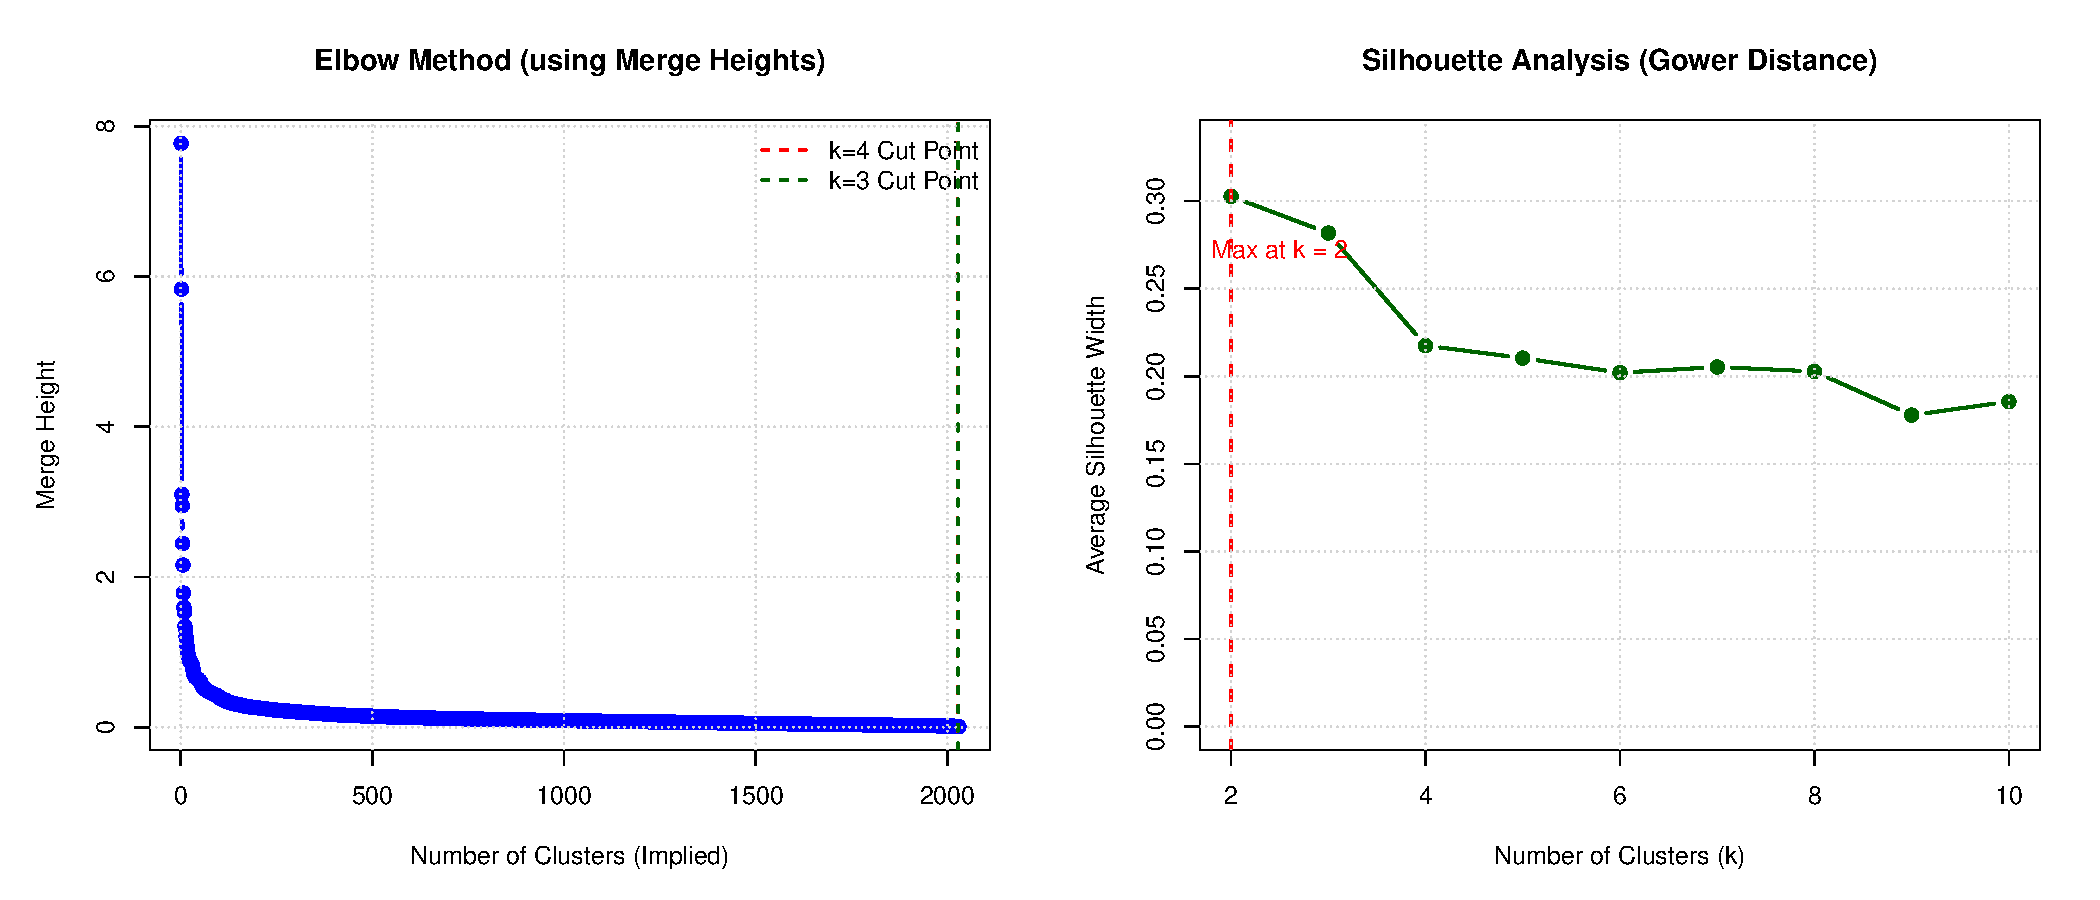
\includegraphics[width=1\linewidth]{Imatges/Clustering_OptimalK_Diagnostics_Gower.pdf}
    \caption{Clustering Optimal Diagnostics}
    \label{fig:optdig}
\end{figure}

The three clusters identified represent distinct customer segments, visualized in Figure \ref{fig:cdend}. Selecting three clusters strikes a balance between statistical validity and practical interpretability—ensuring segments are both mathematically distinct and actionable from a marketing perspective.

\begin{figure}[H]
    \centering
    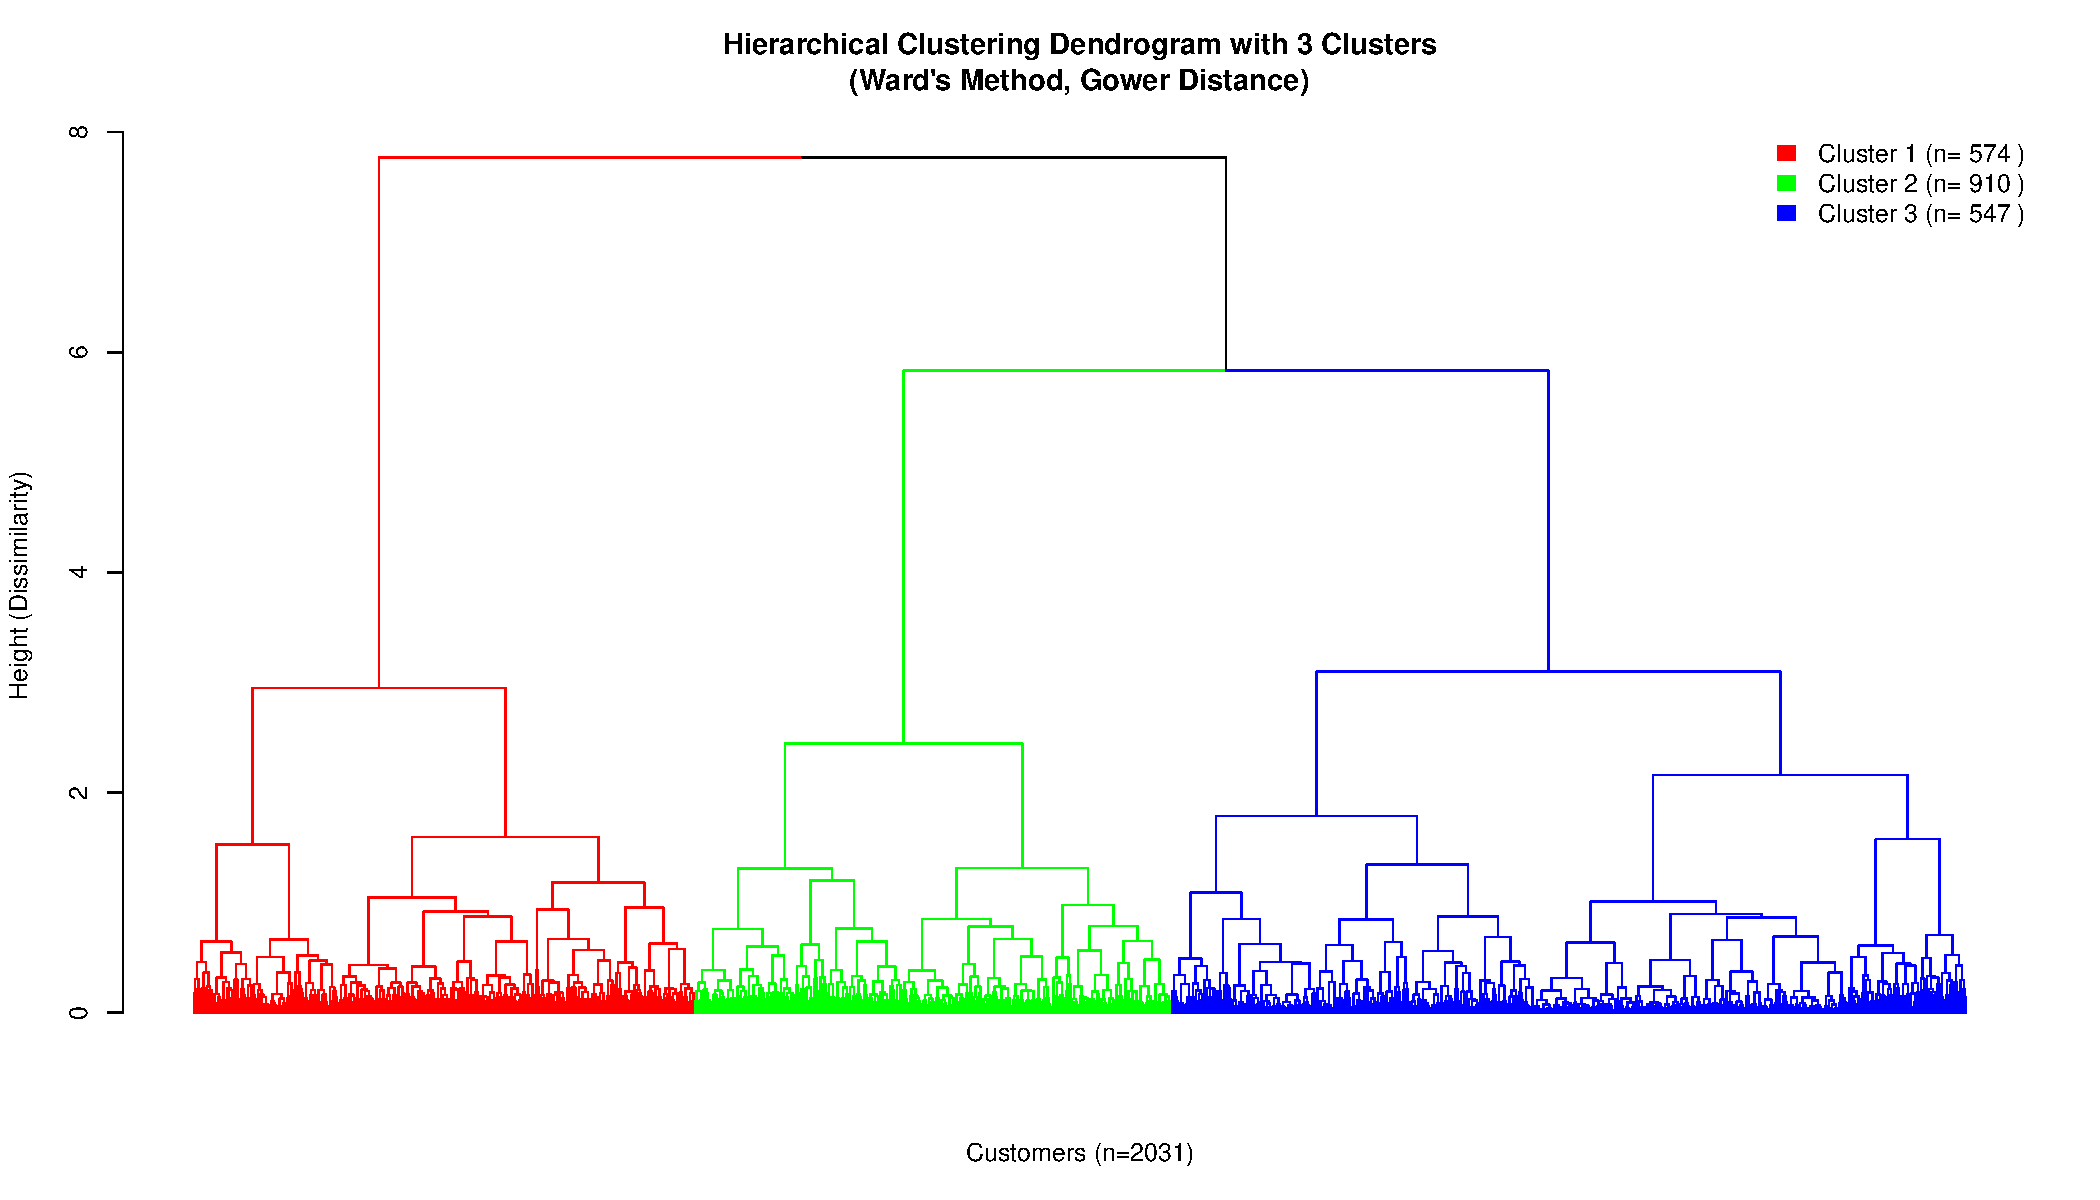
\includegraphics[width=1\linewidth]{Imatges/dendrogram_Gower_Ward_Colored.pdf}
    \caption{Coloured Dendrogram}
    \label{fig:cdend}
\end{figure}


% MICHEL
%%%%%%%%%%%%%%%%%%%%%%%%%%%%%%%%%%%%%%%%%%%%%%%%%%%%%%%%%%%%%%%%%%%%%%%%%%%%%%%%%
\newpage
\raggedright
\section{Profiling}

texto
\newline

\subsection{Education}
Variable Type: Categorical Nominal.\newline
Recall: the Education variable describes the level of studies the consumer has (2nd cycle, Basic, Graduation, Master, PhD).

\begin{figure}[H]
    \centering
    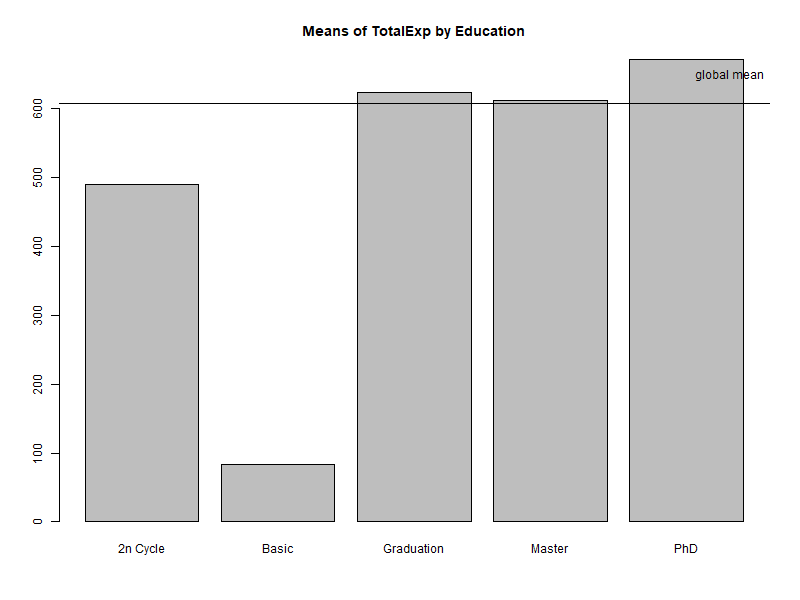
\includegraphics[width=0.8\linewidth]{Imatges/mean_barplot_TotalExp.png}
    \caption{Descripció}
    \label{fig:scree_plot}
\end{figure}
\newline
With a mean barplot we can see the total expent depending on the level of studies, where it is evident that the basic education group spends much less money on their purchase.

\begin{figure}[H]
    \centering
    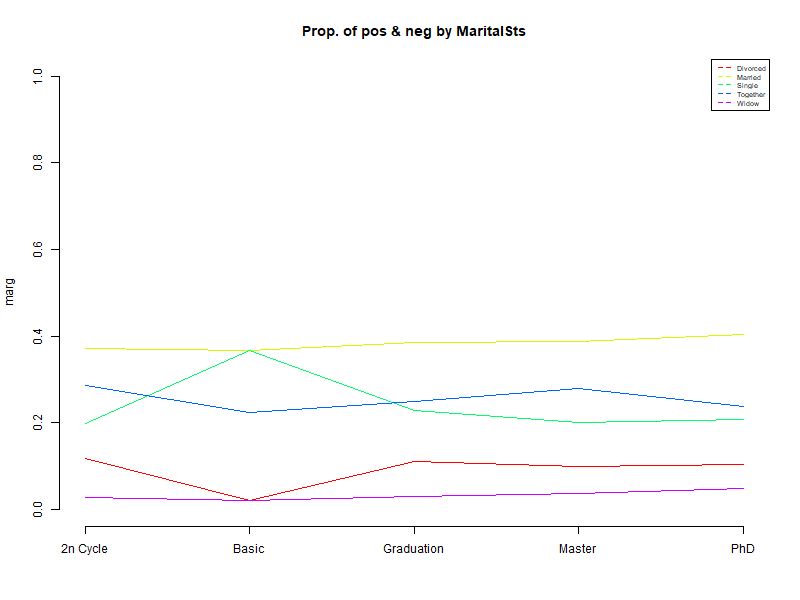
\includegraphics[width=0.8\linewidth]{Imatges/prop_cond_class_MaritalSts_4_legend.png}
    \caption{Descripció}
    \label{fig:scree_plot}
\end{figure}
\newline
Comparing with the marital status we can see that independently of their studies, the customers usualy are married or together. It is worth noting that those with a basic education level are more often married or single.
\begin{figure}[H]
    \centering
    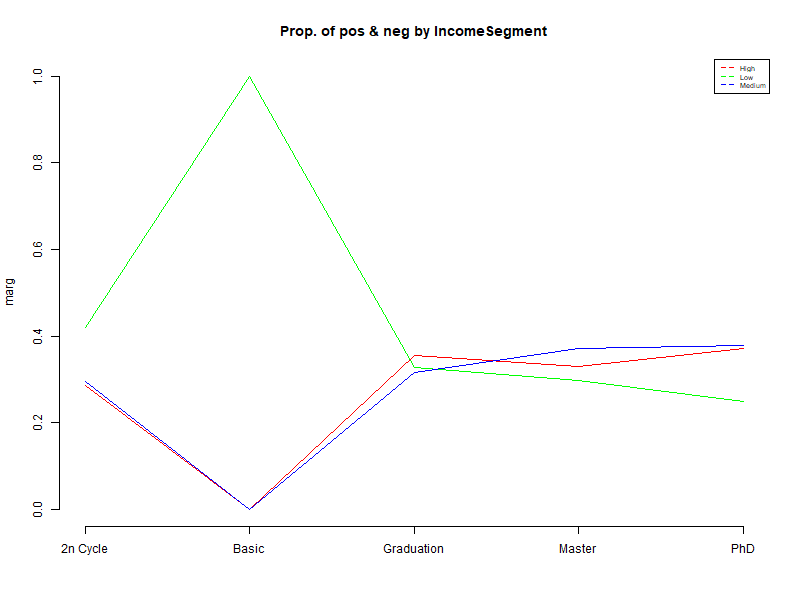
\includegraphics[width=0.8\linewidth]{Imatges/prop_cond_class_IncomeSegment_4_legend.png}
    \caption{Descripció}
    \label{fig:scree_plot}
\end{figure}
\newline
Comparing the income segment we can see that the basic level has the highest frequency with low segment. It shows that they are the ones with the lowest incomes, followed by those with a second-level education, and that there is not much difference among the rest.
\begin{figure}[H]
    \centering
    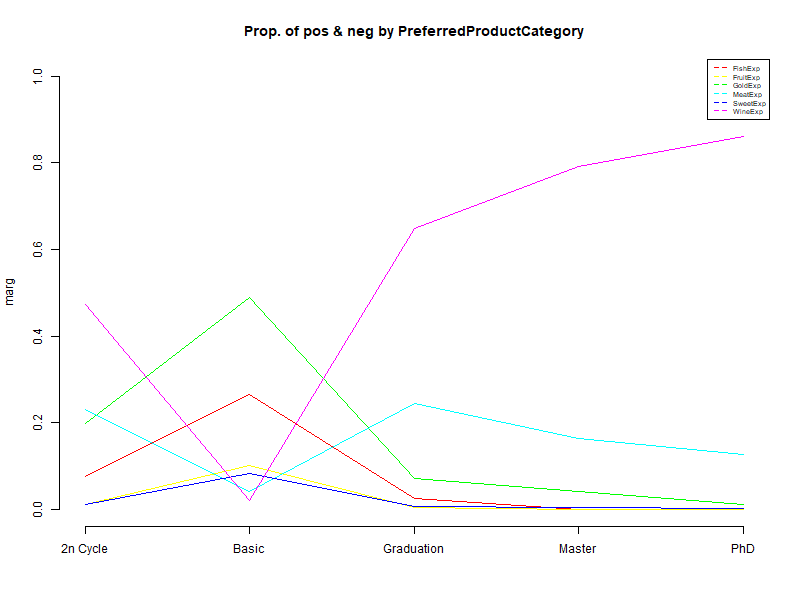
\includegraphics[width=0.8\linewidth]{Imatges/prop_cond_class_PreferredProductCategory_4_legend.png}
    \caption{Descripció}
    \label{fig:scree_plot}
\end{figure}
\newline
About their most purchased product category, we can see that as the level of education increases, there is a tendency to spend more on wine, the customers with lower education levels prefer to buy gold, and those with a graduation level education tend to spend on meat.

\subsection{MaritalSts}
Variable Type: Categorical Nominal.\newline
Recall: the MaritalSts variable describes the marital status of the customer (Divorced, Married, Single, Together, Widow).

\begin{figure}[H]
    \centering
    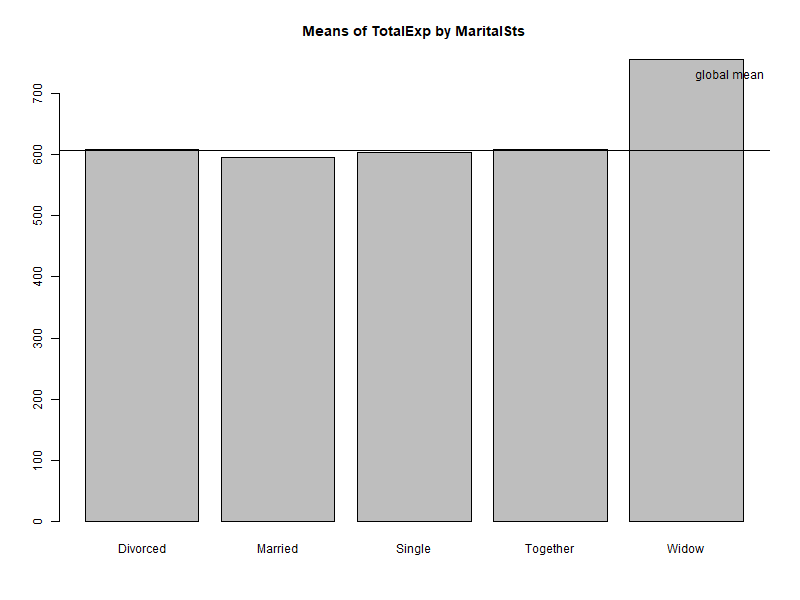
\includegraphics[width=0.8\linewidth]{Imatges/mean_barplot_TotalExp(2).png}
    \caption{Descripció}
    \label{fig:scree_plot}
\end{figure}
\newline
With a mean barplot we can see that the total expenditure by marital status is quite uniform, despite widow customers that spends more on average.

\begin{figure}[H]
    \centering
    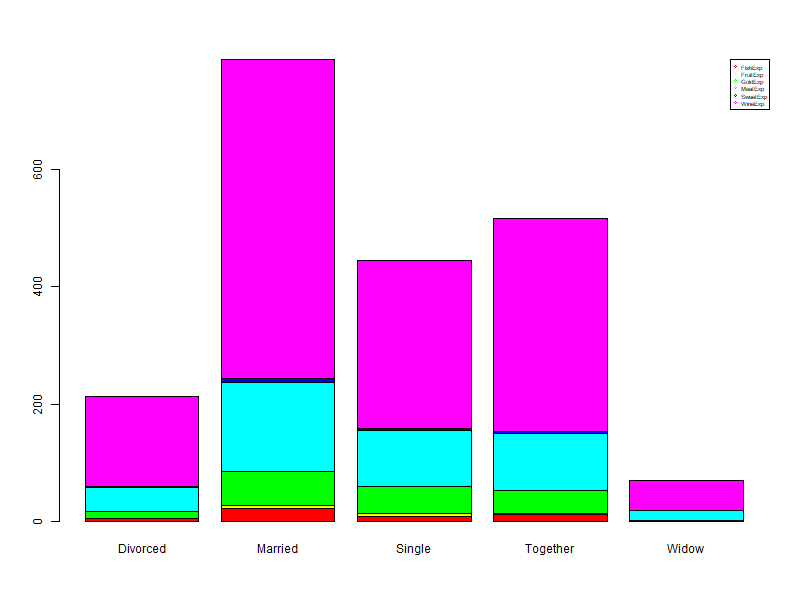
\includegraphics[width=0.8\linewidth]{Imatges/stacked_barplot_counts_PreferredProductCategory_10_legend.png}
    \caption{Descripció}
    \label{fig:scree_plot}
\end{figure}
\newline
It is interesting to observe that regardless of marital status, the main product is wine, followed by meat.

\subsection{IncomeSegment}
Variable Type: Numerical Discrete.\newline
Recall: ...

\begin{figure}[H]
    \centering
    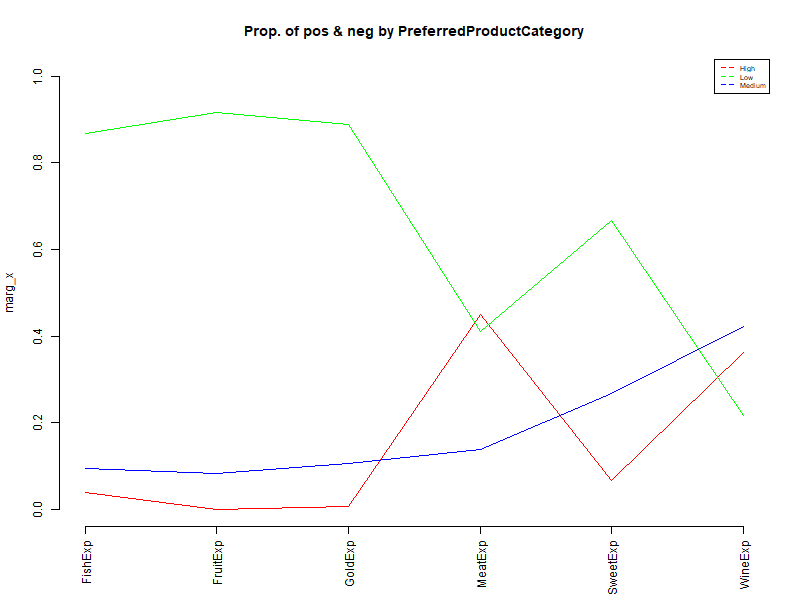
\includegraphics[width=0.8\linewidth]{Imatges/prop_cond_col_var_x_PreferredProductCategory_8_legend.png}
    \caption{Descripció}
    \label{fig:scree_plot}
\end{figure}
\newline
With this graph, it can be observed that the preferred category of customers varies depending on their segment. This shows how different their main interests are when it comes to spending their income.

\subsection{Kidhome}
Variable Type: Numerical Discrete.\newline
Recall: the Kidhome variable describes the number of small children in the customer's household (0 - 5).
\subsection{Teenhome}
Variable Type: Numerical Discrete.\newline
Recall: the Teenhome variable describes the number of teenagers in the customer's household (0 - 5).
\subsection{Response}
Variable Type: Categorical Binary.\newline
Recall: the Response variable describes whether the customer accepted the offer in the last campaign (0 or 1).
\subsection{Complain}
Variable Type: Categorical Binary.\newline
Recall: the Complain variable describes whether the customer has filed a complaint in the last 2 years (0 or 1).
\subsection{HasChildren}
Variable Type: Categorical Binary.\newline
Recall: the HasChildren variable  whether the customer has children or not (0 or 1).

\subsection{PrefereredChannel}
Variable Type: Categorical Nominal.\newline
Recall: the PrefereredChannel variable describes the channel with highest frequency.
\subsection{PrefereredProductCategory}
Variable Type: Categorical Nominal.\newline
Recall: the PrefereredProductCategory variable describes the channel with highest frequency.
\subsection{AccCmp1}
Variable Type: Numerical Discrete.\newline
Recall: 
\subsection{AccCmp2}
Variable Type: Numerical Discrete.\newline
Recall: 
\subsection{AccCmp3}
Variable Type: Numerical Discrete.\newline
Recall: 
\subsection{AccCmp4}
Variable Type: Numerical Discrete.\newline
Recall: 
\subsection{AccCmp5}
Variable Type: Numerical Discrete.\newline
Recall: 



% MARC
%%%%%%%%%%%%%%%%%%%%%%%%%%%%%%%%%%%%%%%%%%%%%%%%%%%%%%%%%%%%%%%%%%%%%%%%%%%%%%%%%
\newpage
\input{conclusions.tex}


% MARC
%%%%%%%%%%%%%%%%%%%%%%%%%%%%%%%%%%%%%%%%%%%%%%%%%%%%%%%%%%%%%%%%%%%%%%%%%%%%%%%%%
\newpage
\input{gant.tex}

\end{document}
